\section{Introduction}

\begin{figure}[t]  
    \centering
    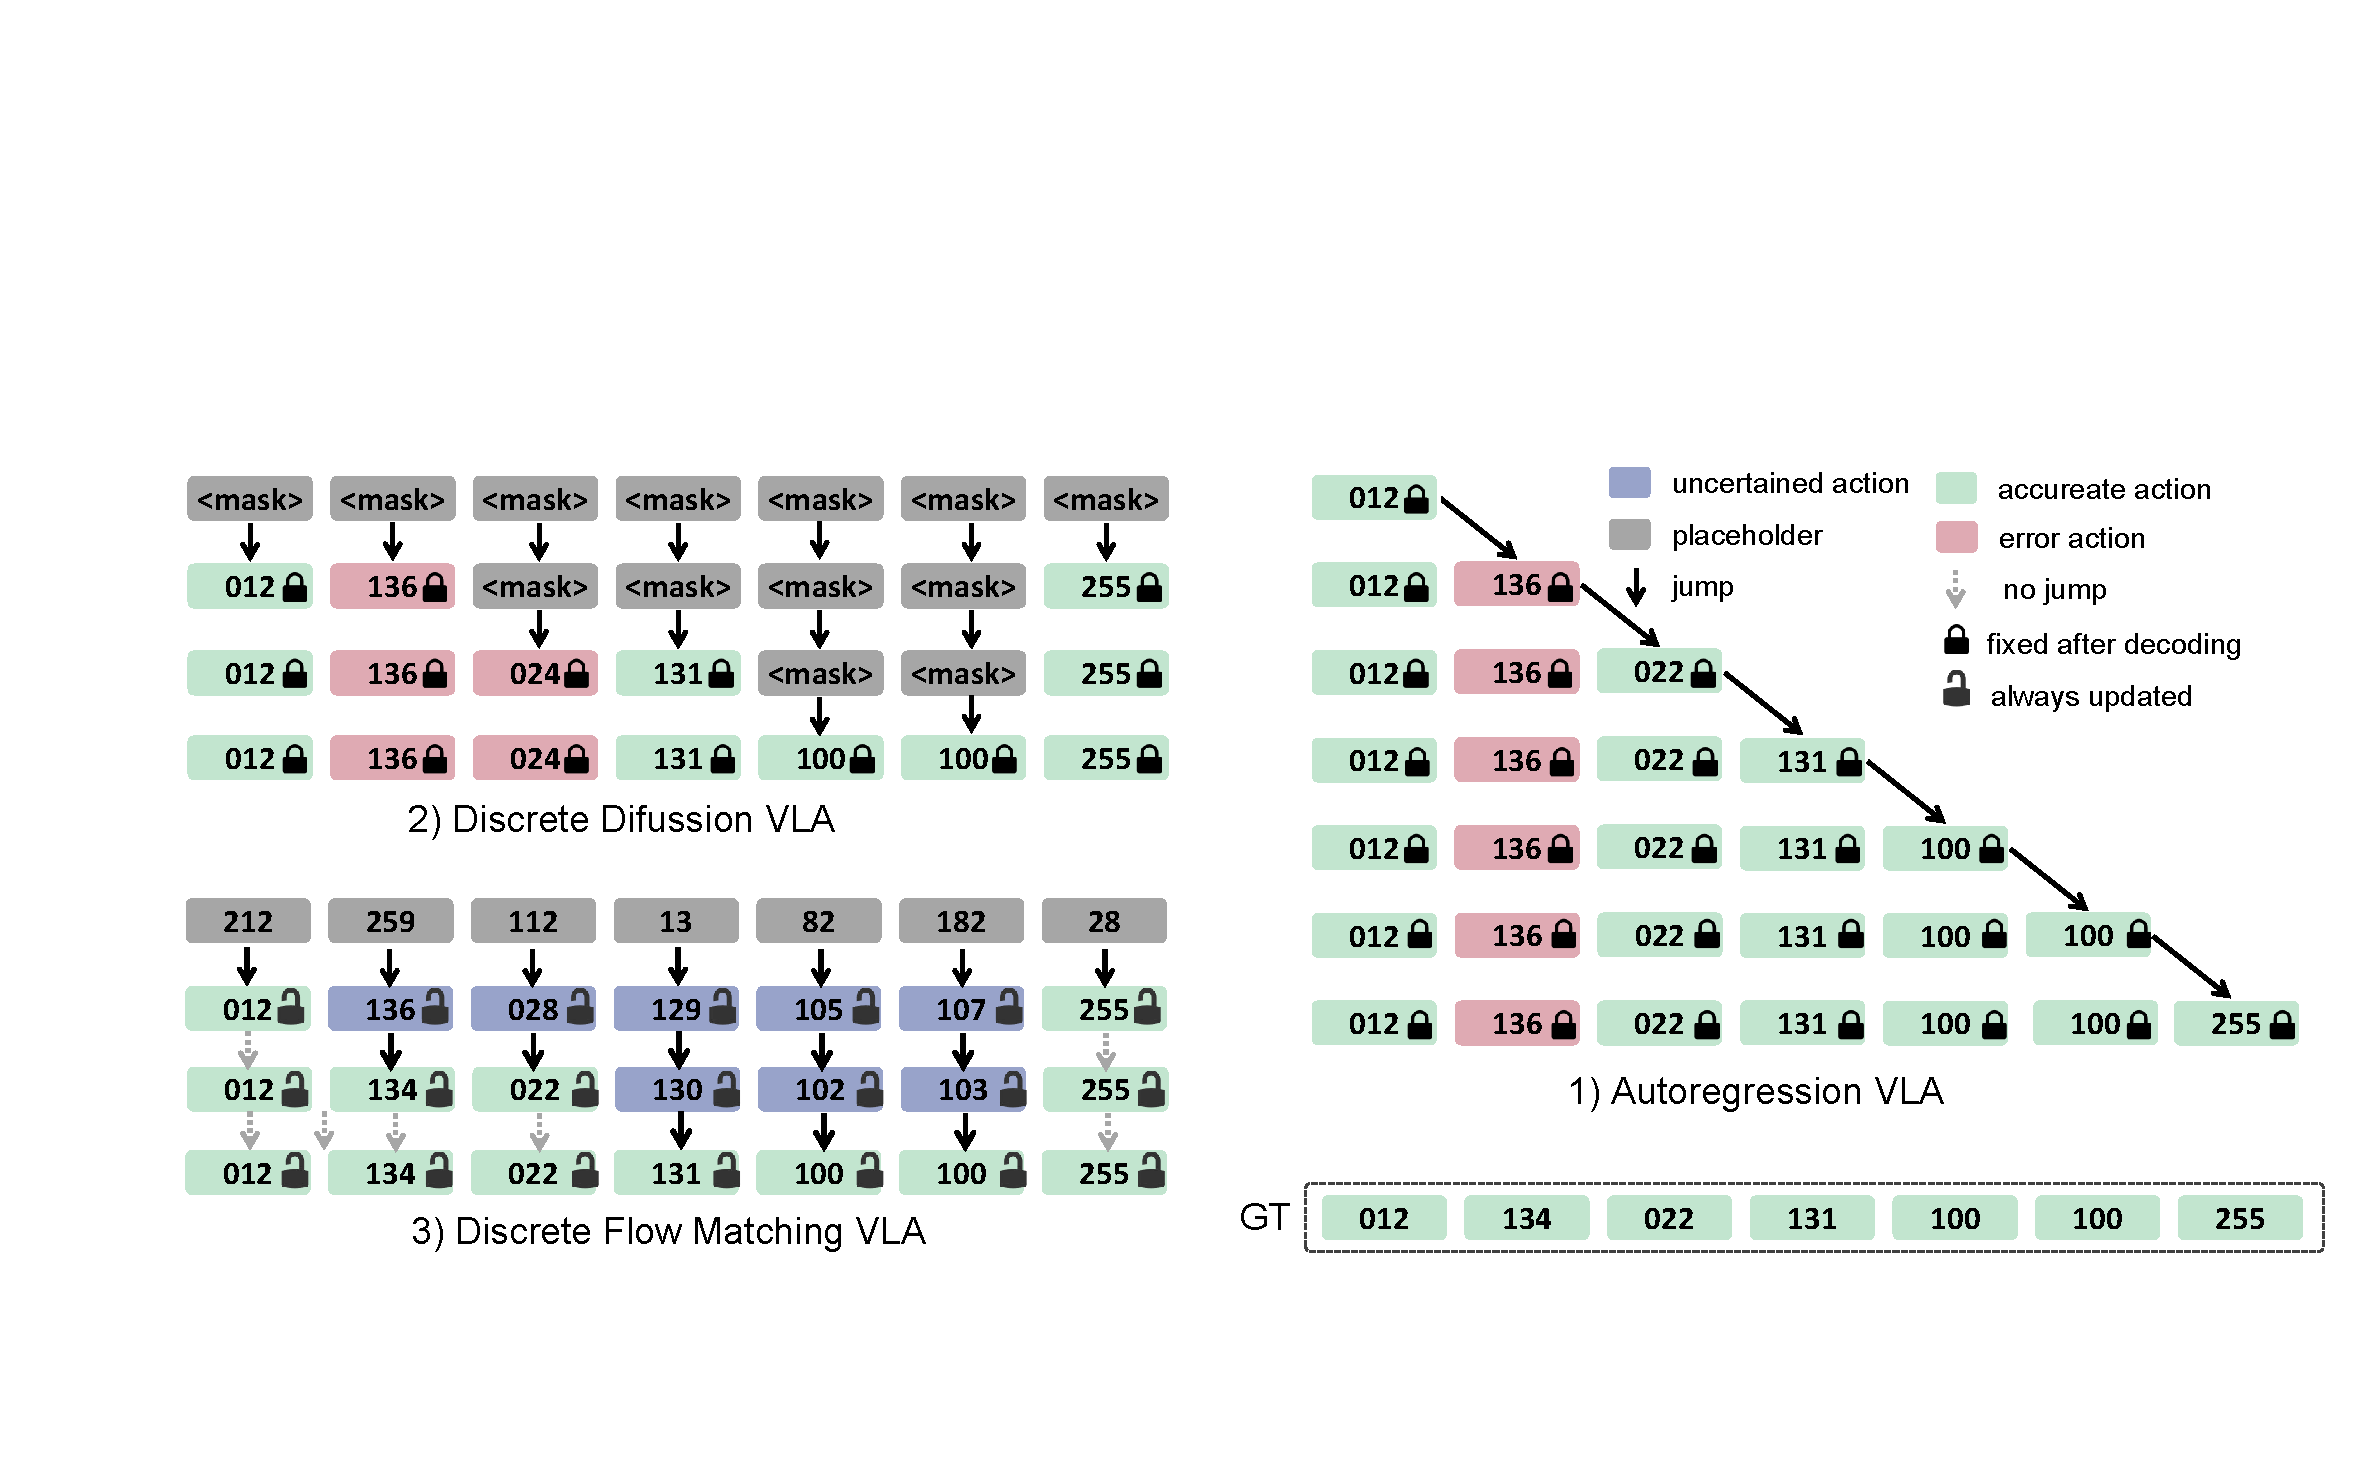
\includegraphics[width=0.98\linewidth]{figure/decode_compare.pdf} 
    \caption{Comparison of decoding paradigms. 1) Autoregressive decoding requires as many steps as the action sequence length, while 2) Discrete Diffusion enables faster generation through parallel token updates. However, both have the same limitation that once an erroneous token is produced, it cannot be corrected in later iterations.
    We refer to this phenomenon as \emph{irreversible commitment}.
    In contrast, 3) our~\method~performs full-sequence action refinement at every iteration, allowing token-level correction and improving action quality for robotic manipulation.}
    \label{fig:decode_compare} 
\end{figure}



Vision--Language--Action (VLA)~\citep{univla,Pi0,gr00t,cui2025openhelix,kim2024openvla,song2025reconvla,wang2025vlaadapter,zhong2026dualcot,yan2026svam} models have become a promising foundation for robotic manipulation, where policies map language instructions and visual observations to executable actions. 
A common and effective design is to discretize actions into tokens, which enables scalable training with Vision-Language Models (VLMs) backbones and leverages their strong capabilities in vision and language
understanding.

Most existing discrete VLA systems fall into two families. Autoregressive (AR) methods~\citep{brohan2022rt,kim2024openvla,univla} decode tokens sequentially with a next-token prediction objective. However, their inherently left-to-right decoding order makes it difficult to revise erroneous tokens once they are emitted.
Discrete diffusion (DD) methods~\citep{song2025accelerating,liang2025discrete,wen2025llada} improve parallelism and often reduce latency, but they may still produce erroneous tokens in early iterations under confidence-guided decoding (see \Cref{fig:decode_compare}).
As a result, AR and DD paradigms struggle with a shared issue in robot control: early decoding errors cannot be effectively corrected and therefore propagate through the action chunk, degrading downstream robotic task performance.
Recent Discrete Flow Matching (DFM)~\citep{wang2025fudoki,luo2025next,havasi2025edit,nguyen2025oneflow,deng2025uniform} studies on Large-Language Models (LLMs) or VLMs have demonstrated competitive performance on text reasoning and editing, as well as image and video generation, by enabling iterative token refinement and flexible generation trajectories guided by velocity field.
These advances inspire us to transfer the same refinement principle to discrete action generation for robotic control.
% Inspired by these advances, we aim to overcome the limitations of AR- and DD-based methods.

We propose \method, a VLA framework that unifies language, vision, and action in a discrete formulation, and employs a discrete action velocity field to enable holistic refinement of action sequences.
As shown in \Cref{fig:decode_compare}, instead of treating action prediction as one-shot token generation, \method~models a token-level probability velocity field and performs iterative full-sequence refinement. This formulation allows the model to repeatedly revisit previously updated positions and selectively correct uncertain tokens as context becomes more informative.
For velocity-field construction, we explore two variants, namely an action-embedding-guided formulation that defines semantically structured probability paths and derives kinetic-optimal velocities, and an auxiliary velocity head formulation that predicts velocities from model hidden states.
For decoding, we adopt a two-stage strategy consisting of an iterative refinement stage for exploration and correction, followed by a deterministic validation stage for stable convergence.

We evaluate \method~on CALVIN, LIBERO, and real-world manipulation tasks. Across benchmarks, \method~consistently improves robot manipulation quality while maintaining strong inference efficiency. Ablation studies further indicate that the proposed design is robust to key scheduler settings, training data scale, and two-stage decoding allocation.

Our contributions are summarized as follows:
\begin{itemize}
    \item We identify the \emph{irreversible commitment} problem in existing autoregressive and discrete diffusion VLA decoding, which limits token correction in robot manipulation.
    \item We propose \method, a discrete flow matching VLA framework that performs iterative full-sequence action refinement via token-level velocity.
    \item We propose two strategies for velocity field construction, namely an action-embedding-guided formulation and an auxiliary velocity head formulation, and we systematically analyze these design variants.
    \item We demonstrate strong empirical performance on CALVIN, LIBERO, and real-world tasks, with consistent gains in both action quality and inference efficiency.
\end{itemize}

\begin{figure*}[t]  
    \centering
    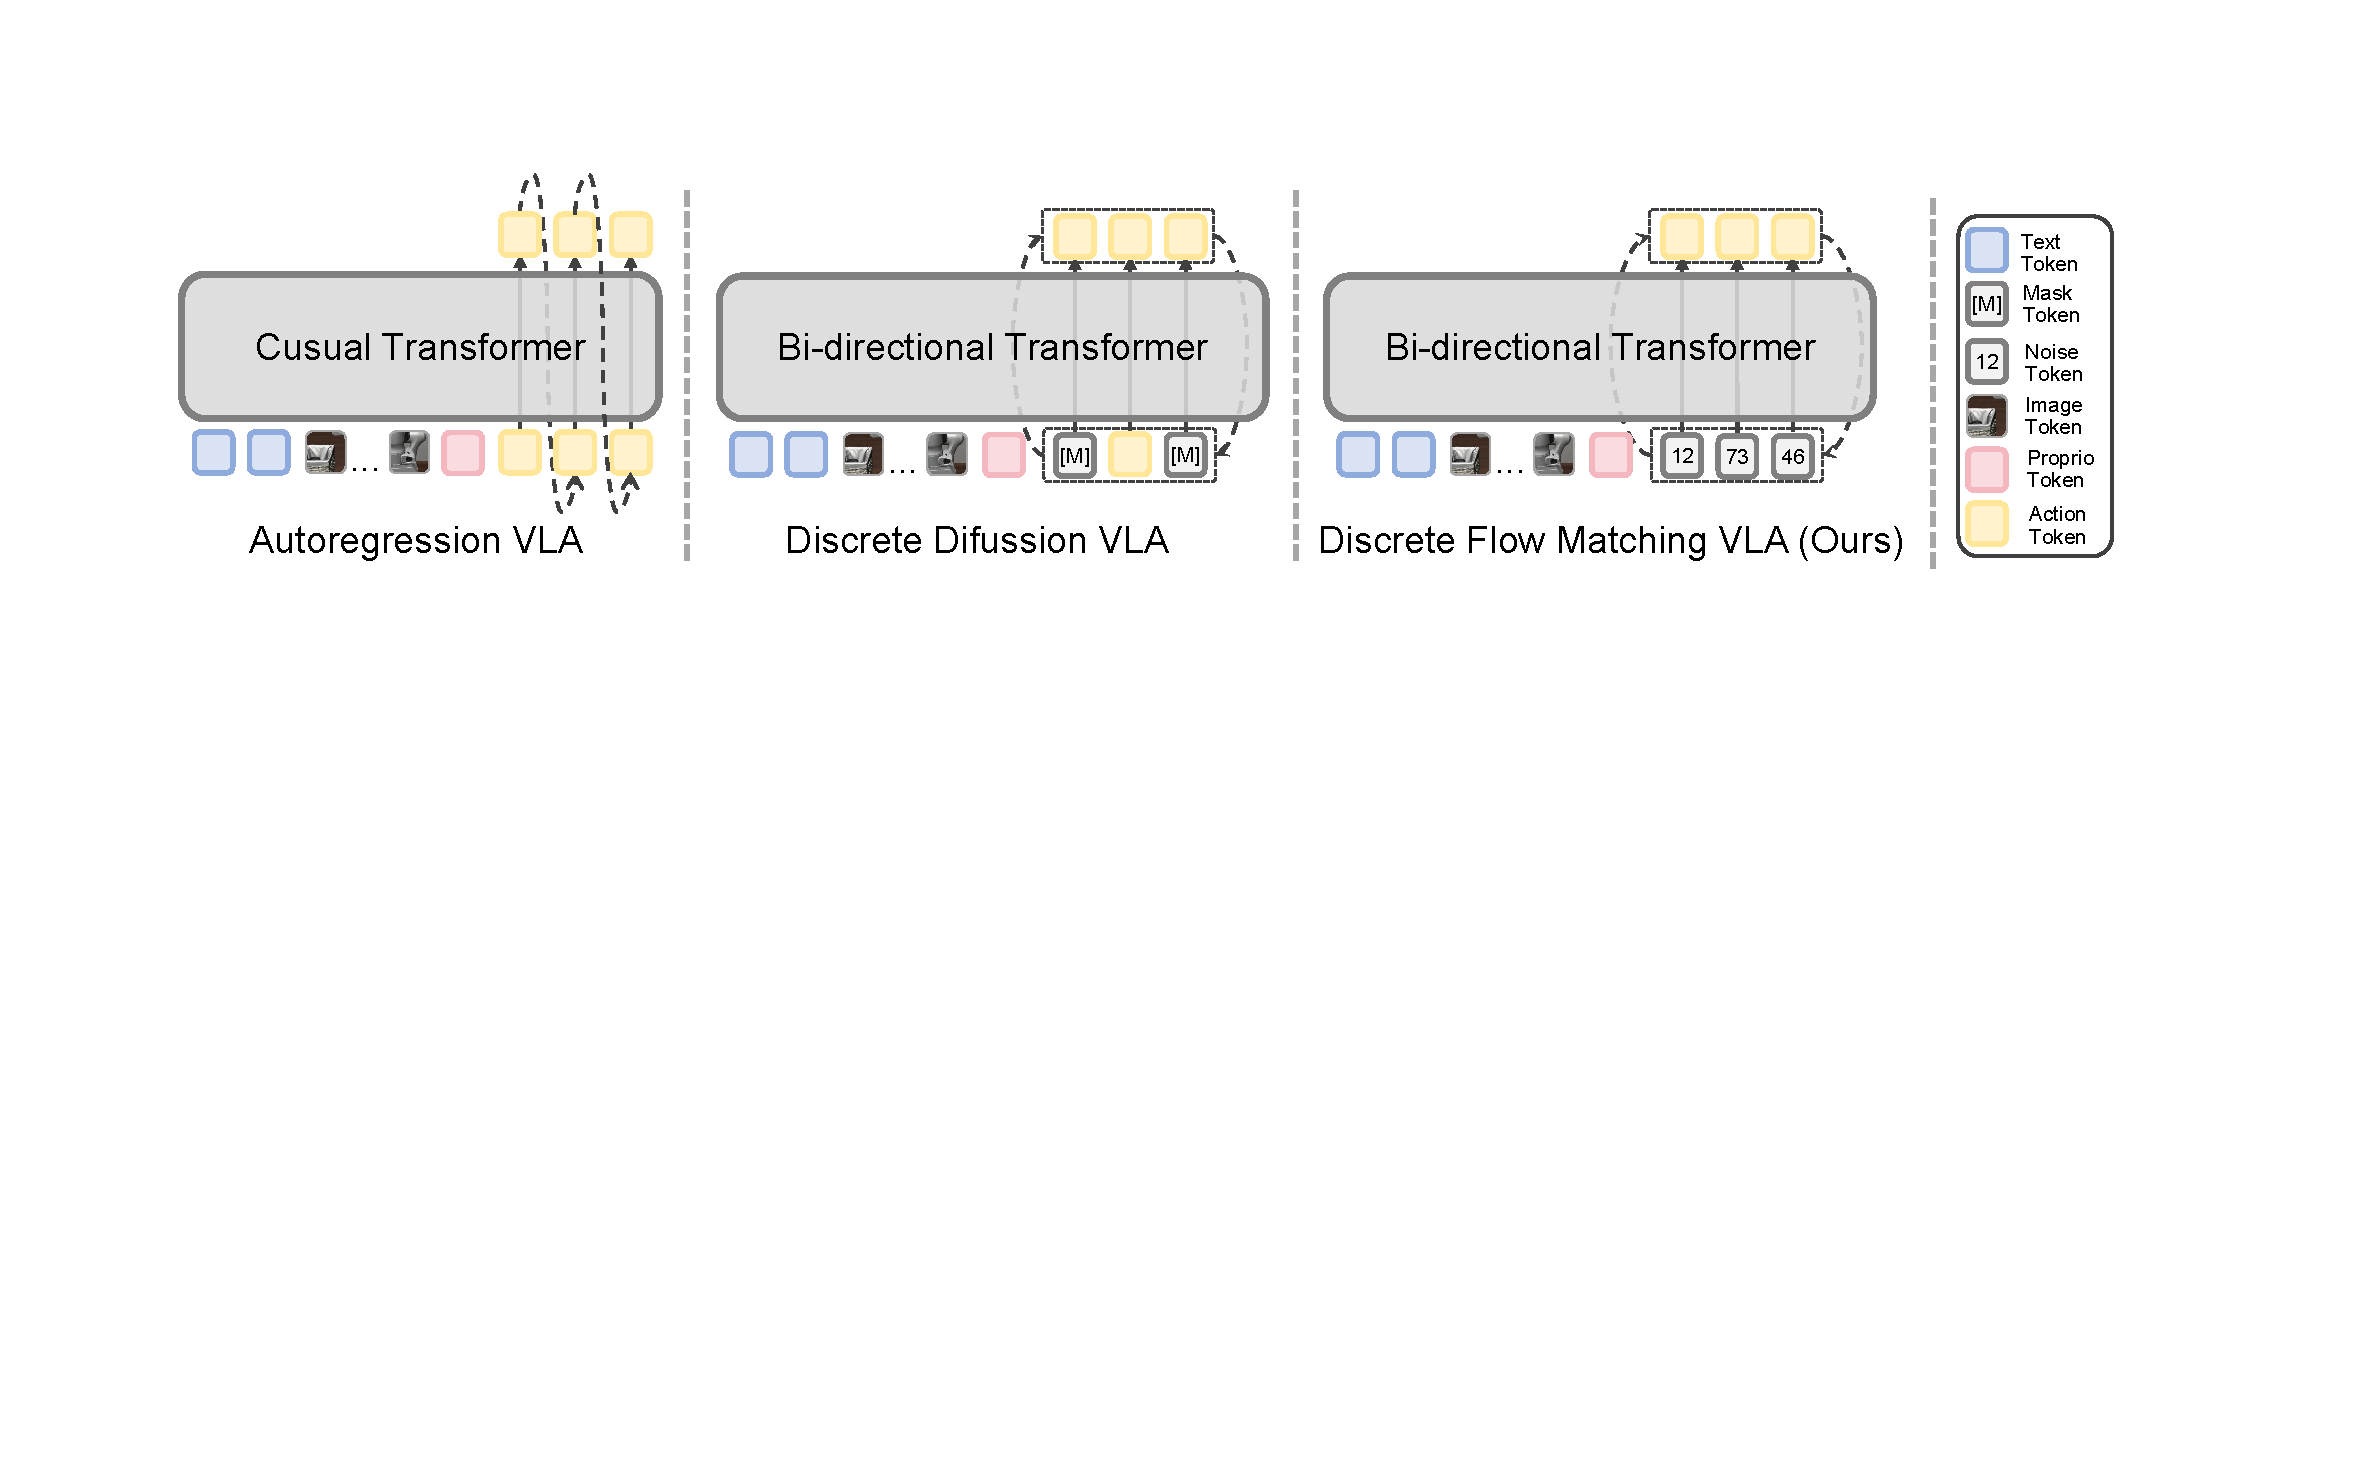
\includegraphics[width=0.98\linewidth]{figure/method_compare.pdf} 
    \caption{Comparison of three discrete VLA paradigms. 
    AR VLA uses causal attention to generate future action tokens from previously generated ones, DD-VLA decodes only masked tokens, while DFM-VLA iteratively refines tokens over the full sequence.
    }
    \label{fig:method_compare}
\end{figure*}
